\let\negmedspace\undefined
\let\negthickspace\undefined
\documentclass[journal]{IEEEtran}
\usepackage[a5paper, margin=10mm, onecolumn]{geometry}
%\usepackage{lmodern} % Ensure lmodern is loaded for pdflatex
\usepackage{tfrupee} % Include tfrupee package

\setlength{\headheight}{1cm} % Set the height of the header box
\setlength{\headsep}{0mm}     % Set the distance between the header box and the top of the text

\usepackage{gvv-book}
\usepackage{gvv}
\usepackage{cite}
\usepackage{amsmath,amssymb,amsfonts,amsthm}
\usepackage{algorithmic}
\usepackage{graphicx}
\usepackage{textcomp}
\usepackage{xcolor}
\usepackage{txfonts}
\usepackage{listings}
\usepackage{enumitem}
\usepackage{mathtools}
\usepackage{gensymb}
\usepackage{comment}
\usepackage[breaklinks=true]{hyperref}
\usepackage{tkz-euclide} 
\usepackage{listings}
% \usepackage{gvv}                                        
\def\inputGnumericTable{}                                 
\usepackage[latin1]{inputenc}                                
\usepackage{color}                                            
\usepackage{array}                                            
\usepackage{longtable}                                       
\usepackage{calc}                                             
\usepackage{multirow}                                         
\usepackage{hhline}                                           
\usepackage{ifthen}                                           
\usepackage{lscape}
\begin{document}

\bibliographystyle{IEEEtran}
\vspace{3cm}

\title{NCERT-6.5.14}
\author{EE24BTECH11065 - Spoorthi yellamanchali
}
% \maketitle
% \newpage
% \bigskip
{\let\newpage\relax\maketitle}

\renewcommand{\thefigure}{\theenumi}
\renewcommand{\thetable}{\theenumi}
\setlength{\intextsep}{10pt} % Space between text and floats


\numberwithin{equation}{enumi}
\numberwithin{figure}{enumi}
\renewcommand{\thetable}{\theenumi}


\textbf{Question:}
\\
Find two positive numbers $x$ and $y$ such that $x + y$ = 60 and $xy^3$ is maximum.\\
\\
\textbf{ Theoretical Solution: }
\\
From the question, we can write,
\begin{align}
        y = 60 - x
\end{align}
On substituting equation $\brak{0.1}$ in $xy^3$, we get,
\begin{align}
    x\brak{60 - x}^3
\end{align}
On differentiating equation $\brak{0.2}$ with respect to $x$ and equating it to zero, we get,
\begin{align}
    \brak{60 - x}^3 - 3x\brak{60 - x}^2 = 0\\
    \brak{60 - x}^2\brak{60 - 4x} = 0
\end{align}
From the equation $\brak{asd}$, we get , $x = 60$ and $x = 15$,\\
On differentiating equation $\brak{asd}$, with respect $x$, and substituting both values of $x$, we get,
\begin{align}
    -3\brak{60 - x}^2 -3\brak{60 - x}^2 + 6x\brak{60 - x}\\
    \therefore \frac{d^2y}{dx^2} = \brak{60 - x}\brak{-360 + 12x}
\end{align}
On substituting $x = 15$, we get ,
\begin{align}
    \frac{d^2y}{dx^2} < 0 
\end{align}
that means, $xy^3$ is maximum when $x = 15$, then , $y = 60 - 15=45$\\
$\therefore$ $xy^3$ is maximum when $x = 15$ and $ y = 45$.\\
\\ 
\textbf{Solution using gradient descent method.}
\\
The gradient descent(in case of finding minima) or the gradient ascent method(in case of finding maxima) is a computational algorithm which optimizes and maximises/minimizes the functional curve.\\
It uses the concept of gradient or slope to do so as we know the fact that slope or gradient is zero or almost negligible at points of maxima and minima.\\
It works by itertively adjusting the input variable $x$ in the direction of function's gradient.\\
starting from initial guess $x_0$,the algorithm iteratively updates $x$ using the rule\\

\begin{align}
    x_{new} = x_{current} + \alpha \times f^\prime\brak{x_{current}}
\end{align}

Here $\alpha$ is the learning rate which controls the size of each step.\\
The iteration stops when the change in $x$ between iterations becomes smaller than a predefined tolerance.\\
We know that, in our question,
\begin{align}
    f^\prime \brak{x} = -3x\brak{60-x}^2 + \brak{60-x}^3
\end{align}
On substituing equation $\brak{0.9}$ in $\brak{0.8}$ , we get,
\begin{align}
    x_{new} = x_{current} + \alpha\brak{-3x_{current}\brak{60-x_{current}}^2 + \brak{60-x_{current}}^3}
\end{align}
and by taking,
\begin{align}
    \alpha = 0.000001\\
\end{align}
And convergence = $1e-6$\\
initial guess $x_0$ = 14.0,
We get,\\
x value at maxima =  14.999878397267214\\
y value at maxima =  45.00012160273279 \\ 
 \textbf{Solution using geometric programming:}\\
Geometric programming is a type of mathematical optimization that is used for problems where the objective and constraints can be expressed as posynomials or monomials.\\
\\ A monomial is a product of variables raised to constant powers. A monomial is of the form:
${x_1}^{a_1}{x_2}^{a_2}{x_3}^{a_3}.....{x_n}^{a_n}$\\
where $x_1,x_2,x_3.....x_n$ are the variables and $a_1,a_2,a_3....a_n$ are the real constant powers(can be positive or negative or zero.)\\

 posynomial is a sum of monomials, where each monomial in the sum has non-negative coefficients. A posynomial is of the form:
 \begin{align}
     f\brak{x_1,x_2,x_3...,x_n} = c_1{x_1}^{a_{11}}{x_2}^{a_{12}}...{x_n}^{a_{1n}} + c_2{x_1}^{a_{21}}{x_2}^{a_{22}}....{x_n}^{a_{2n}} + .....+ c_n{x_1}^{a_{n1}}{x_2}^{a_{n2}}...{x_n}^{a_{nn}}
 \end{align}
 Where $c_i\geq 0$ (non-negative constants)\\
 The equation above is the expression of the objective function which we wish to maximise or minimise.\\
 \\ The constraints of the problem are typically posynomials, and they are usually represented as:
 \begin{align}
     g_i\brak{x_1,x_2,x_3....x_n} \leq 0 ; i = 1,2,3...m.
 \end{align}
 $g_i\brak{x_1,x_2,x_3....x_n}$ is a posynomial.\\
Maximization of a Posynomial Objective Function:
\begin{align}
    f\brak{x_1,x_2,x_3...,x_n} = \sum c_ix_1^{a_{i1}}x_2^{a_{i2}}...{x_n}^{in}
\end{align}
Subject to constraints of the form:
\begin{align}
    g_i\brak{x_1,x_2,x_3....x_n} \leq 0;\ i = 1,2,3...,m
\end{align}
The objective function in our problem is
\begin{align}
    f\brak{x,y} = xy^3
\end{align}
To apply Geometric Programming, we take the logarithm of both the objective function and the constraint.\\
This step simplifies the problem and makes it easier to handle by converting products into sums.\\
For the objective $f\brak{x,y} = xy^3$, we take the natural logarithm:\\
\begin{align}
    \ln{xy^3} = \ln{x} + 3\ln{y}
\end{align}

The constraint is $x + y = 60$.\\
Taking logarithm of this constraint directly is not meaningful, as it is a sum , not a product.\\
we will simply proceed with it as it is since it's already linear and suitable for GP.\\
In order to combine objective and constraint we use lagrange multipliers\\
Lagrangian combines the objective function and the constraint by introducing a Lagrange multiplier $\lambda$ for the constraint.\\
Lagrangian for an objective function $f\brak{x,y}$ and constraint $g\brak{x,y}$ is given by:
\begin{align}
    L\brak{x,y,\lambda} = f\brak{x,y} + \lambda\brak{g\brak{x,y}}
\end{align}
we can take our objective function to be $\ln{x} + 3\ln{y}$ as , since $ln$ is an increasing function, $\ln{xy^3}$ is maximized whenever $xy^3$ is maximized.
$\therefore$ On applying lagrangian for equation $\brak{d}$ and $\brak{a}$, we get,
\begin{align}
    L\brak{x,y,\lambda} = \ln{x} + 3\ln{y} + \lambda\brak{x - y - 60}
\end{align}
To find the optimal solution, we take the partial derivatives of the Lagrangian with respect to $x$, $y$, and $\lambda$, and set them equal to zero.\\

On partially derivating equation $\brak{a}$ with respect to $x$:
\begin{align}
    \frac{\partial L}{\partial x} = \frac{1}{x} - \lambda = 0\\
    \lambda = \frac{1}{x}
\end{align}
On partially derivating equation $\brak{a}$ with respect to $y$:
\begin{align}
    \frac{\partial L}{\partial y} = \frac{3}{y} - \lambda\\
    \lambda = \frac{3}{y}
\end{align}
On partially derivating equation $\brak{a}$ with respect to $\lambda$:
\begin{align}
    \frac{\partial L}{\partial \lambda} = 60 - x + y = 0\\
    x + y = 60
\end{align}
From the first two equations, we can equate $\lambda$:
\begin{align}
    \frac{1}{x} = \frac{3}{y}
\end{align}
Solving for $y$ in terms of $x$, we get:
\begin{align}
    y = 3x
\end{align}

Now substitute $y = 3x$ into the constraint $x + y =60$ , then , we get,
\begin{align}
    x + 3x = 60\\
    x = 15\\
    y = 45
\end{align}
$\therefore$ $x = 15$ and $y = 45$ at maxima.
On solving for values of $x$ and $y$ using a python function , we get\\
value for $x$ using geometric programming 14.99878409289183\\
value for $y$ using geometric programming 45.00121536318684.\\
Due to floating-point rounding errors, the computed solution will be an approximation, leading to slight deviations.

\begin{figure}[h!]
   \centering
   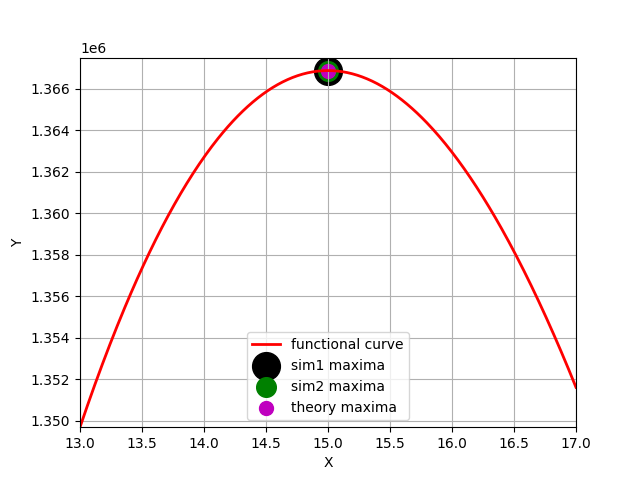
\includegraphics[width=0.75\columnwidth]{figures/Figure_1.png}
   \label{graph of the function}
\end{figure}

\end{document}


